\chapter{Data and Experimental Setup}
\label{ch:setup}

\section{Datasets}

\paragraph{SisFall.} The archive contains 4{,}505 trial files from 23 young adults (SA, 19--30 years)
and 15 elderly volunteers (SE, 60--75 years). Elderly participants performed ADL only, with one
exception: SE06, a judo expert, also simulated the 15 fall types. Every fall in the dataset was
therefore performed by a healthy person, and all but 75 of the 1{,}798 fall files by someone under
31. ADL trials last 10--100\,s (180\,s for a few long recordings); fall trials last 15\,s. No sample
was missing and none exceeded the $\pm16\,g$ range.

\paragraph{Daphnet.} Seventeen recordings from ten patients with idiopathic Parkinson's disease
(mean age 66.4 years), mostly recorded off medication to provoke freezing \parencite{bachlin2010daphnet}. The
archive provides both a CSV re-export and the original UCI release; we use the original text files.
Timestamps are integer milliseconds and alternate between 15 and 16\,ms, i.e.\ \SI{64.00}{\hertz} on
average. Two patients (S04, S10) never froze. In S10, 6.3 annotated minutes contain trunk readings of
exactly $(0,0,0)$\,mg, which is physically impossible since gravity alone produces about 1000\,mg;
these segments are sensor dropouts and are removed; kept, they would count as normal walking.

\begin{table}[ht]
\centering
\small
\caption{Windows after preprocessing. SisFall training fall windows include the 0.25\,s-grid copies.}
\label{tab:data}
\begin{tabular}{llrrrr}
\toprule
Domain & Split & Subjects & Negatives & Positives & Positive (\%) \\
\midrule
SisFall & train & 25 & 44{,}705 & 4{,}877 & 9.84 \\
SisFall & validation & 5 & 8{,}738 & 229 & 2.55 \\
SisFall & test & 8 & 14{,}173 & 381 & 2.62 \\
Daphnet & all (zero-shot) & 10 & 15{,}676 & 1{,}734 & 9.96 \\
\bottomrule
\end{tabular}
\end{table}

\paragraph{Subject split.} SisFall training: SA01--SA15 and SE01--SE10 (including SE06). Validation:
SA16--SA18, SE11, SE12. Test: SA19--SA23, SE13--SE15. Elderly volunteers in the validation and test
sets contribute only negatives, which makes the false-alarm estimate representative of older users.

\begin{figure}[ht]
\centering
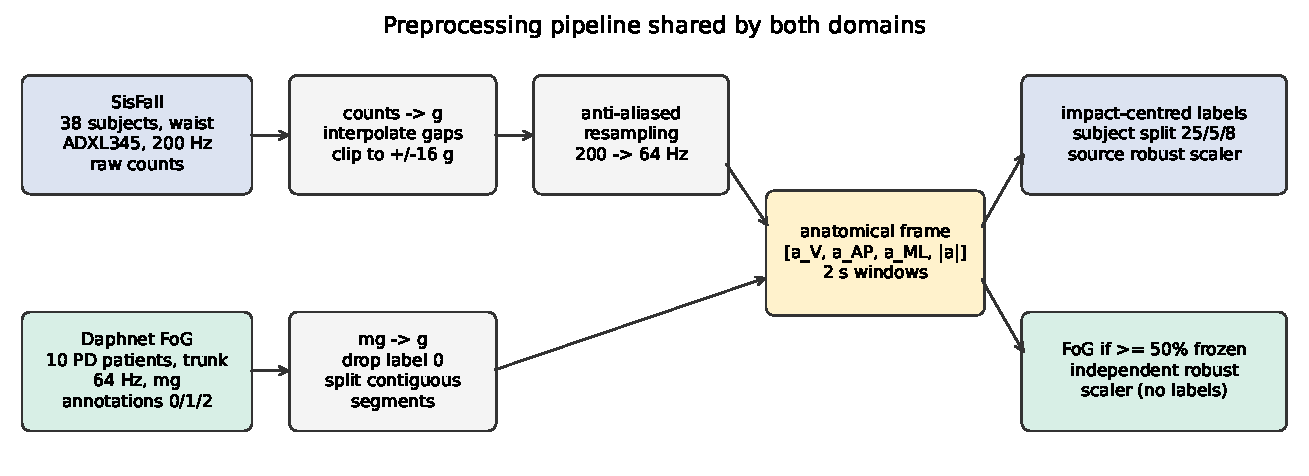
\includegraphics[width=\textwidth]{fig01_pipeline}
\caption{Preprocessing shared by both domains. Only the population and the target event differ
between the two branches.}
\label{fig:pipeline}
\end{figure}

\section{Exploratory analysis}
\label{sec:eda}

\paragraph{Axis identification.} \Cref{fig:axes} confirms the data-driven frame: walking puts
$0.97\,g$ on the vertical axis, and the static acceleration after a fall moves to $a_{AP}=-0.60\,g$
for forward falls and $+0.83\,g$ for backward falls, i.e.\ prone and supine, as the sign convention
predicts. The small negative AP offset during walking ($-0.2\,g$) shows that the SisFall logger was
tilted on the belt by roughly 12 degrees, a reminder that ``the waist'' is not one orientation.

\begin{figure}[ht]
\centering
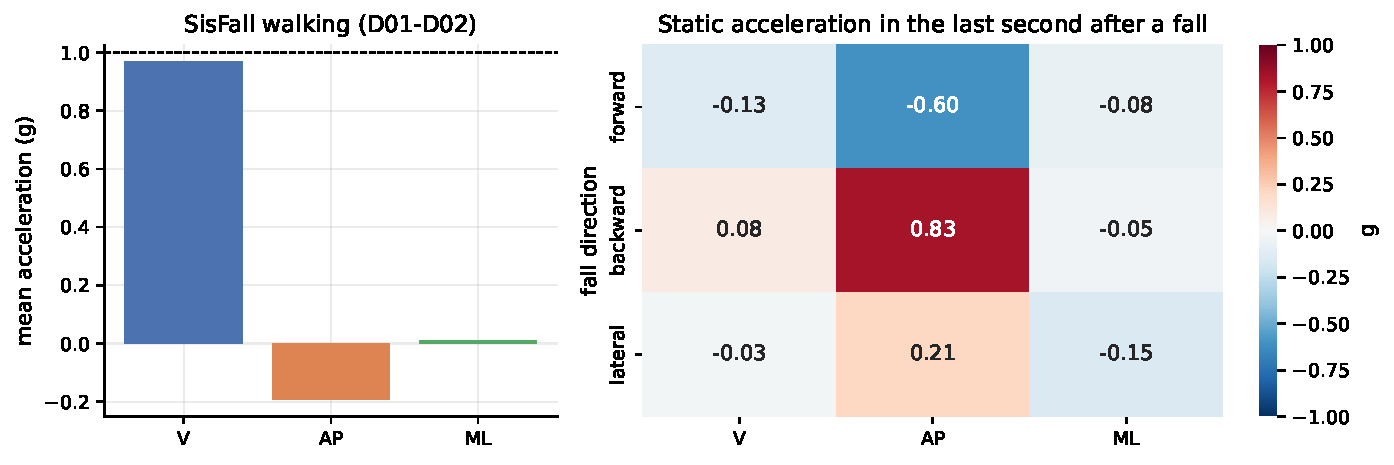
\includegraphics[width=0.95\textwidth]{fig03_axis_identification}
\caption{Left: mean acceleration per anatomical axis during SisFall walking. Right: static acceleration
in the last second of fall trials, grouped by the fall direction given in the dataset documentation.}
\label{fig:axes}
\end{figure}

\paragraph{Signal morphology.} A SisFall fall is a short, violent transient followed by rest in a new
orientation (\Cref{fig:sisfall-signal}). At the trunk, a Daphnet freeze looks very different: the
gait rhythm becomes irregular and small, fast oscillations appear, but nothing comparable to an
impact occurs (\Cref{fig:daphnet-signal}). The ankle shows the trembling more clearly than the trunk,
which is why the freeze index is usually computed at the shank.

\begin{figure}[ht]
\centering
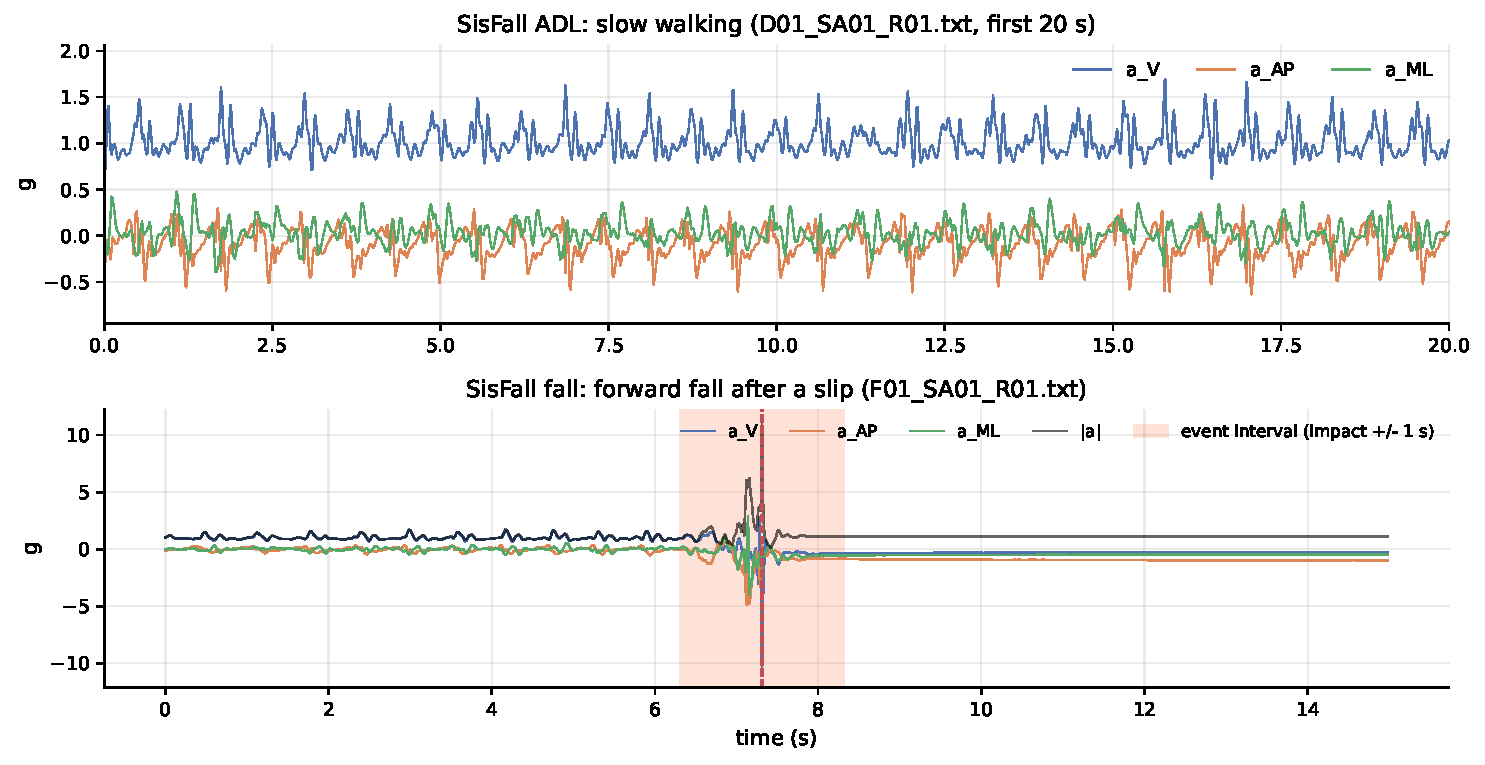
\includegraphics[width=\textwidth]{fig04_sisfall_signals}
\caption{SisFall in the common frame. Top: slow walking. Bottom: forward fall after a slip; the shaded
band is the event interval used for labelling and the dashed line the detected impact.}
\label{fig:sisfall-signal}
\end{figure}

\begin{figure}[ht]
\centering
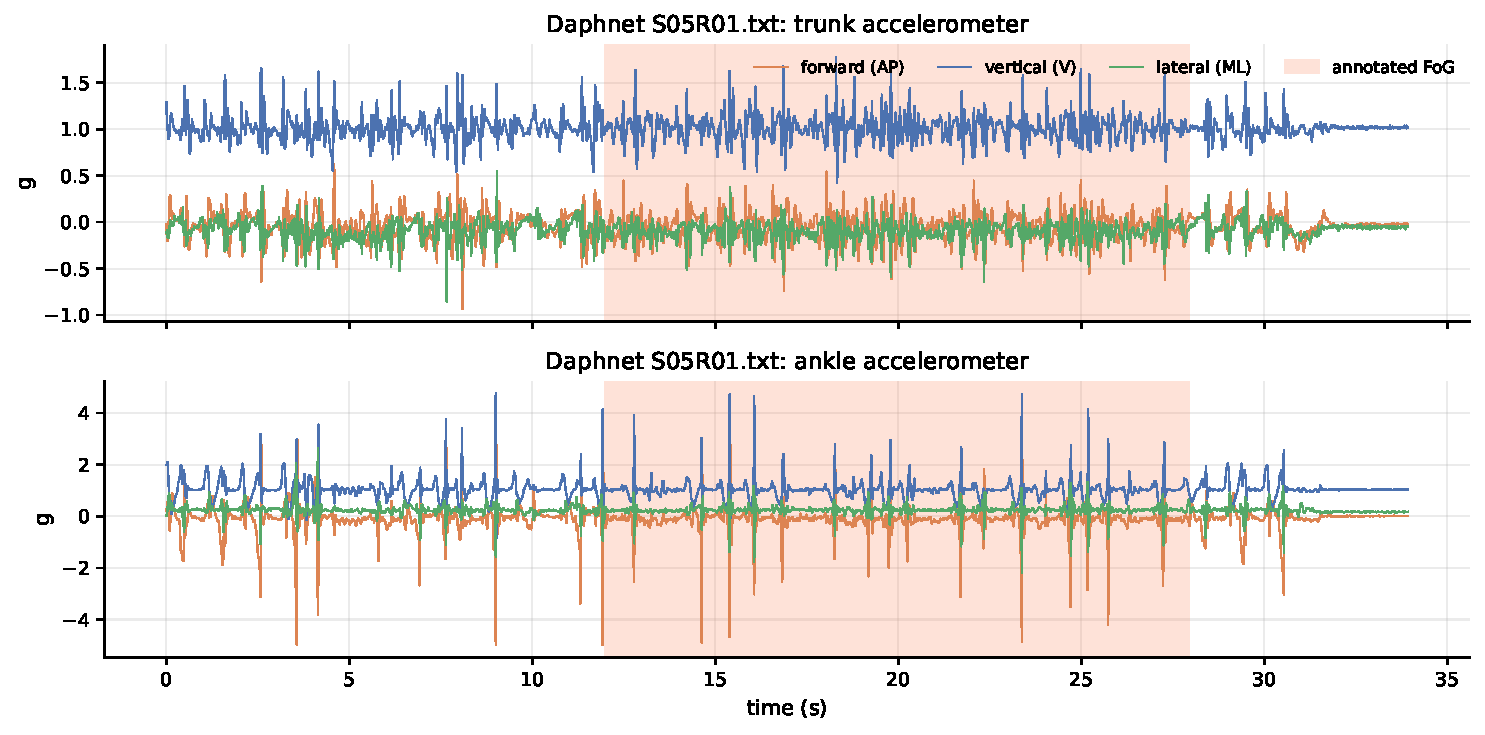
\includegraphics[width=\textwidth]{fig05_daphnet_signals}
\caption{Daphnet recording with the longest freezing episode, trunk (used by the models) and ankle
(for reference). The shaded band is the clinical FoG annotation.}
\label{fig:daphnet-signal}
\end{figure}

\paragraph{Descriptors and spectra.} \Cref{fig:descriptors} and \Cref{tab:mannwhitney} quantify the
difference. A fall window has a median peak of $5.6\,g$ and a $|a|$ standard deviation thirteen times
that of ADL (rank-biserial $r=0.94$ and $0.82$). FoG windows differ from Parkinsonian walking much less:
a factor of two in $|a|$ variability, $0.2\,g$ in peak and $+0.3$ in log freeze index, all with moderate
effect sizes ($r=0.33$--$0.37$). The largest difference between the two \emph{normal} classes, healthy
ADL and Parkinsonian walking, is spectral: the freeze index is higher in Daphnet ($r=0.42$) while
amplitudes are almost identical. In the frequency domain
(\Cref{fig:psd}), falls raise the power at every frequency by about two orders of magnitude, while FoG
adds a bump between 3 and 8\,Hz. The positive classes of the two domains barely overlap: in raw
window statistics, falls form an isolated cluster, whereas FoG windows share most of their
neighbourhoods with walking windows (\Cref{fig:tsne-raw}). This is the first piece of evidence that the transfer problem is dominated by
concept shift.

\begin{figure}[ht]
\centering
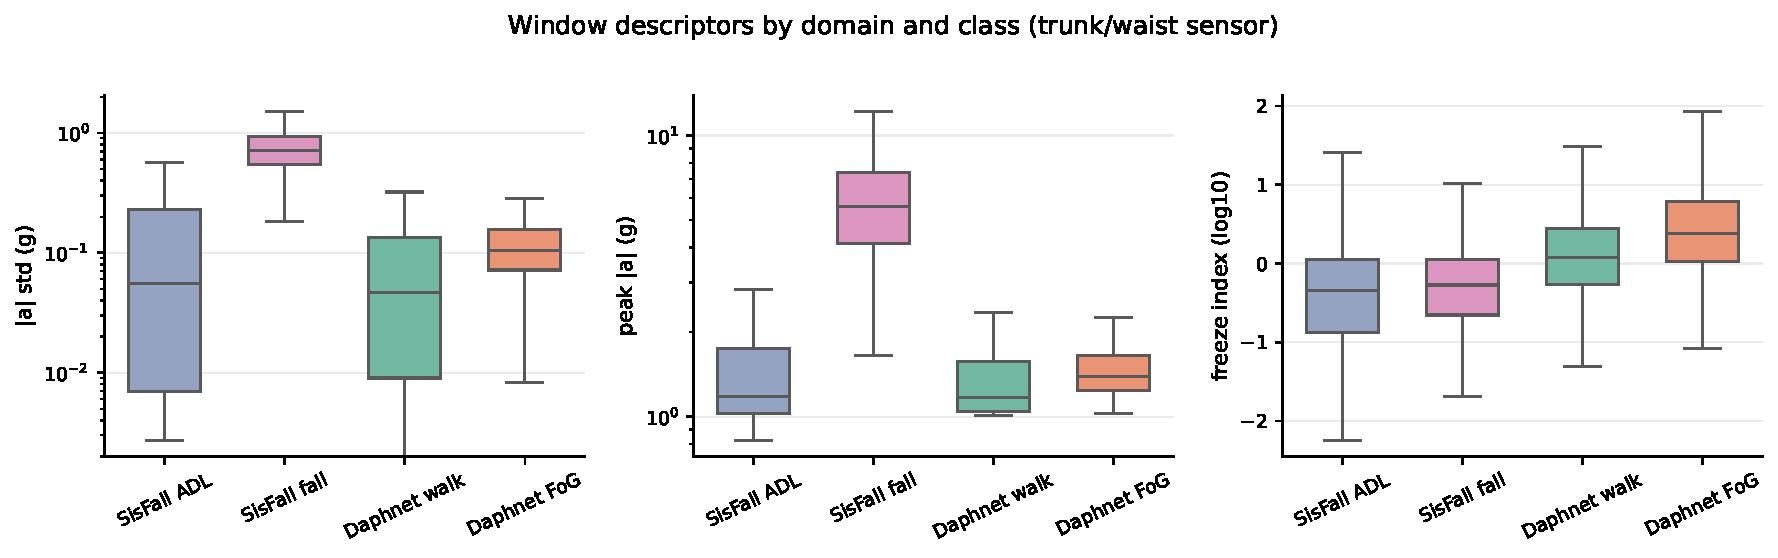
\includegraphics[width=\textwidth]{fig06_window_descriptors}
\caption{Window descriptors (random subsets of up to 6{,}000 windows per group; outliers hidden).
The freeze index is computed on the AP axis.}
\label{fig:descriptors}
\end{figure}

\begin{table}[ht]
\centering
\small
\caption{Window descriptors: medians and Mann--Whitney rank-biserial effect size $r$ (all $p<10^{-10}$ unless stated).}
\label{tab:mannwhitney}
\begin{adjustbox}{max width=\textwidth}
\begin{tabular}{llrrr}
\toprule
Comparison (A vs B) & Descriptor & Median A & Median B & $r$ \\
\midrule
SisFall ADL vs SisFall fall & $|a|$ std (g) & 0.055 & 0.714 & 0.82 \\
 & peak $|a|$ (g) & 1.179 & 5.575 & 0.94 \\
 & freeze index (log10) & -0.338 & -0.273 & 0.09 ($p=2.5e-08$) \\
Daphnet walk vs Daphnet FoG & $|a|$ std (g) & 0.047 & 0.104 & 0.37 \\
 & peak $|a|$ (g) & 1.172 & 1.389 & 0.34 \\
 & freeze index (log10) & 0.077 & 0.381 & 0.33 \\
SisFall ADL vs Daphnet walk & $|a|$ std (g) & 0.055 & 0.047 & -0.04 ($p=2.1e-05$) \\
 & peak $|a|$ (g) & 1.179 & 1.172 & 0.01 ($p=5.9e-01$) \\
 & freeze index (log10) & -0.338 & 0.077 & 0.42 \\
\bottomrule
\end{tabular}
\end{adjustbox}
\end{table}

\begin{figure}[ht]
\centering
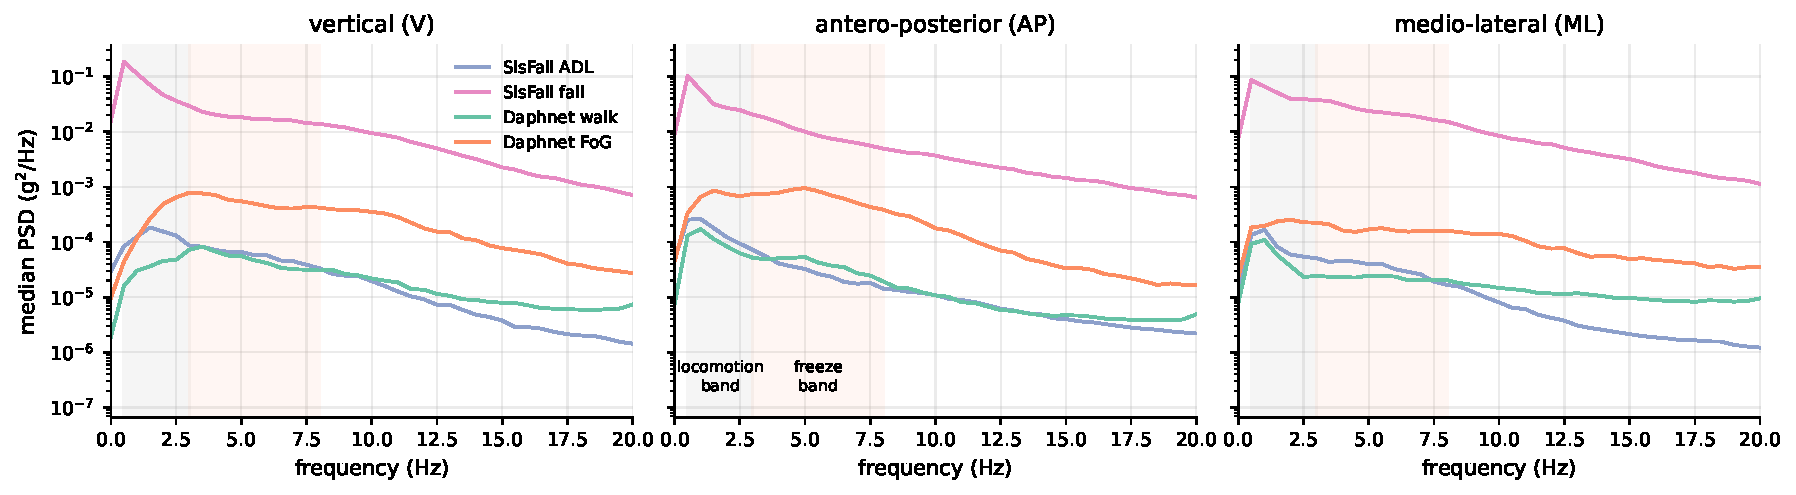
\includegraphics[width=\textwidth]{fig07_power_spectra}
\caption{Median Welch power spectral density per group and axis (mean removed per window). Grey:
locomotion band; orange: freeze band.}
\label{fig:psd}
\end{figure}

\begin{figure}[ht]
\centering
\begin{subfigure}{0.48\textwidth}
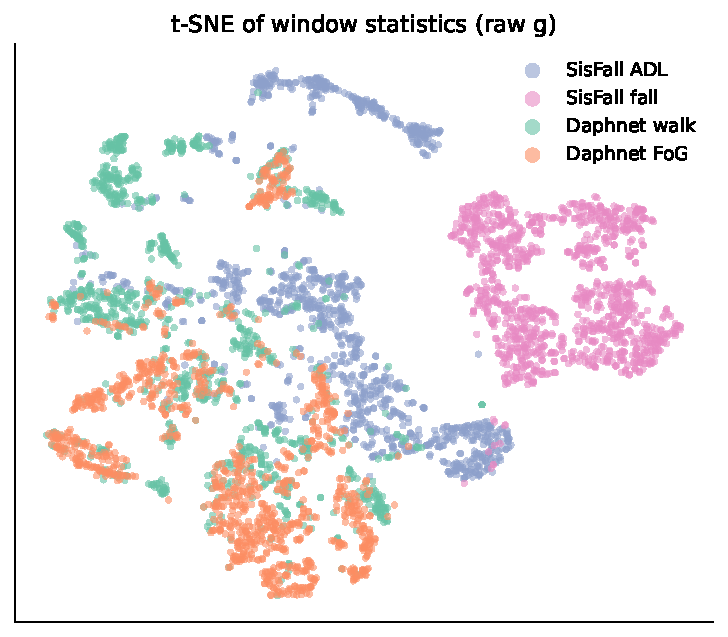
\includegraphics[width=\textwidth]{fig10_tsne_raw_features}
\caption{t-SNE of window statistics.}
\label{fig:tsne-raw}
\end{subfigure}\hfill
\begin{subfigure}{0.48\textwidth}
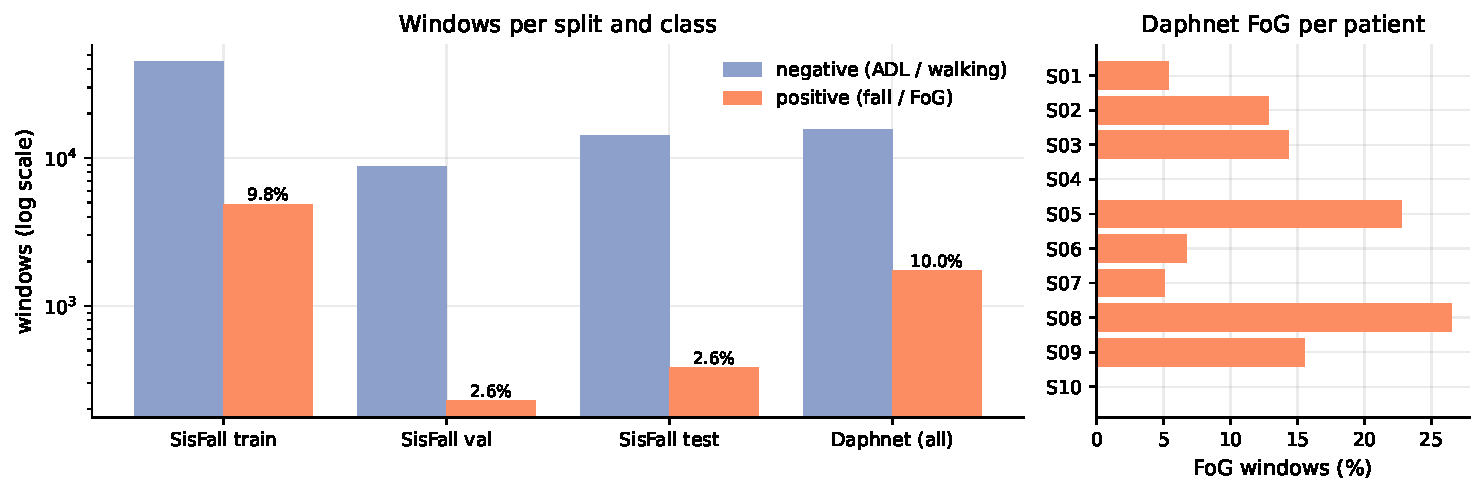
\includegraphics[width=\textwidth]{fig02_class_balance}
\caption{Class balance per split.}
\end{subfigure}
\caption{Left: hand-crafted window statistics (per-channel mean, standard deviation, percentiles and
the descriptors above) embedded with t-SNE. Right: windows per split and class (log scale) and FoG
prevalence per Daphnet patient.}
\end{figure}

\paragraph{Amplitude distributions and scaling.} Raw per-channel distributions of healthy ADL and
Parkinsonian walking are already close (\Cref{fig:amplitude}, left), because both are dominated by
upright posture. Scaling with source statistics leaves Daphnet much narrower than SisFall on the
vertical and magnitude channels; scaling each domain with its own statistics widens Daphnet to unit
inter-quartile range, which brings the walking distributions closer but also amplifies the small
FoG oscillations. Daphnet values are stored with a resolution of about 10\,mg against 3.9\,mg for the
ADXL345, another (minor) difference between the sensors.

\begin{figure}[ht]
\centering
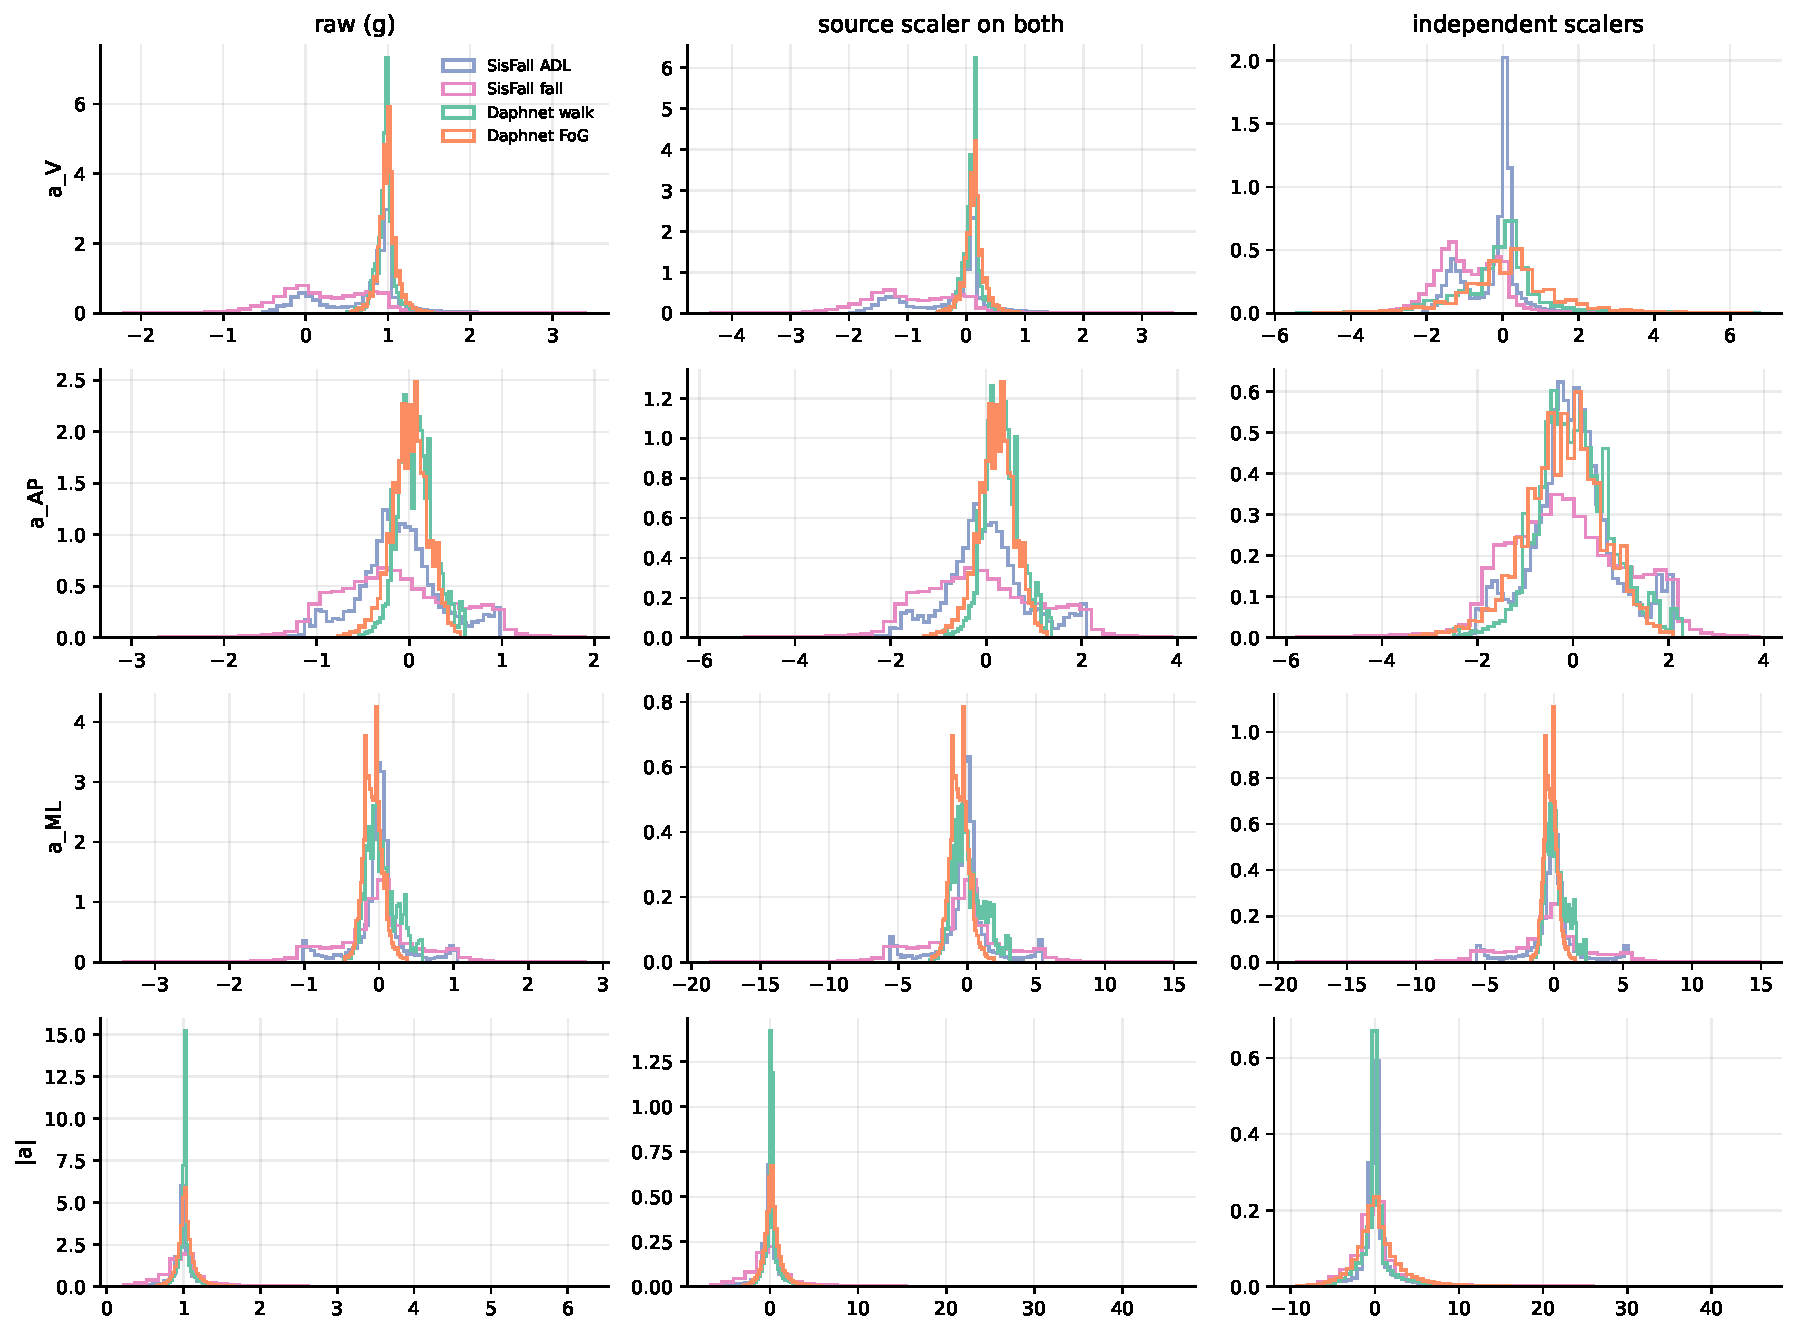
\includegraphics[width=\textwidth]{fig08_amplitude_distributions}
\caption{Per-channel sample distributions in raw units, with the source scaler applied to both domains,
and with independent per-domain scalers.}
\label{fig:amplitude}
\end{figure}

\section{Implementation}

Everything is implemented in PyTorch \parencite{paszke2019pytorch} and executed end to end in six
Jupyter notebooks (data preparation, exploratory analysis, hyper-parameter search, training and
zero-shot evaluation, target adaptation, shift analysis). Shared components (models, training loop,
metrics) live in a small \texttt{src} package so that the notebooks call identical code. Network
training (notebooks 03--05) ran on one NVIDIA T4 GPU; preprocessing, inference from the saved
checkpoints and all analyses also run on a two-core CPU, where they reproduce the reported metrics.
The training cost per epoch is given in \Cref{tab:hparams}.
Each checkpoint stores the weights together with the configuration, the scaler statistics and the
validation threshold, so it is self-contained for inference.
